\section{Inserting devices}
This section contains the description of the functionality related solution regarding adding devices to a WorkCell. The solution was heavily inspired by the XMLRWLoader from the loaders section of the RobWork library. The solution was put in a class called loader.

\subsection{General explanation of the solution}
The solution for the requirements related to insertion of devices (See need to have requirement 3) was, just like with inserting frames and geometries, divided into two parts. The first part is the interface to the user required for the user to be able to supply the necessary information needed. The interface is explained later in section~\ref{sec:DeviceTab}. The second part is the process of creating and inserting the device defined by the user. The reason for this separation is the same as the one given in inserting frames and geometries section (section~\ref{subsec:iFramesAGeomsGE}).

\subsection{Using the loader}
The loader contains two functionalities the user should be aware of. The first functionality is a function called add. This functions adds the device described in a XML file to a given WorkCell. The function add takes in a string representing the path to the, the WorkCell which the information should be added to, a string representing the custom name of the device and a string containing the name of the frame on which the device should be placed. The user can also supply a transform which is applied to the base frame of the device, giving it an initial placement. The transform can be supplied in two different ways, the user can supply the function with a transform object or the x, y, z and R, P, Y values.\\
The loader also contains the functionality to load a WorkCell from an XML-file, just like the XMLRWLoader. This functionality was made solely to give the loader more consistency in its functionalities.\\
An example of using the loader to add a device can be seen on figure~\ref{fig:UseCodeExampleLoader}.

\begin{figure}[h]
	\centering
	\lstset{language=C++} 
	\begin{lstlisting}[frame=single]
	WorkCell::Ptr wc; // WorkCell needing the device
	String path = "Some path"; // Path to the device
	String name = "test"; // Custom name given to device
	String parent = "WORLD"; // Name of parent frame
	Transform3D transform; // Initial placement of the device
	
	// Add device with the parameters given
	ei::loader::add(path, wc, name, parent, transform);
	\end{lstlisting}
	\caption{Code example of using the to add a device}
	\label{fig:UseCodeExampleLoader}
\end{figure}


\subsection{Understanding the XMLRWLoader}
In order to understand what it takes to load information from an XML-file into the format used in RobWork, it is worth the time to study the XMLRWLoader. Another good reason to study the XMLRWLoader is that it solves a problem very similar to the problem of interest in this chapter. There are only two differences, the XMLRWLoader loads not only devices and it creates a new WorkCell to put the items in.\\

The function of interest from the XMLRWLoader is the loadWorkcell function. This function takes in a single input which is a string containing the path to the XML file describing the WorkCell.\\
A good place to start is to analyse the flow that the loadWorkCell function have. The function can be seen as a sequence of actions:

\begin{enumerate}
	\item Parse the XML file using parseWorkCell from XMLRWParser contained in the loaders section. This takes in the provided path.
	\begin{enumerate}
		\item The information is parsed into a struct called DummyWorkCell that arranges the information neatly for when it should be used.
	\end{enumerate}
	\item Do sanity check on all the frames
	\begin{enumerate}
		\item Each frame needs to have a valid parent frame
	\end{enumerate}
	\item Create a new WorkCell object
	\item Create and add all the frames, defined in the DummyWorkCell, to the WorkCell
	\begin{enumerate}
		\item Does not include frames from devices
	\end{enumerate}
	\item Add all frame properties to the WorkCell
	\item Create all devices defined in the DummyWorkCell
	\begin{enumerate}
		\item Create and add all device related frames
		\item Create all device related models
	\end{enumerate}
	\item Create and add models, belonging to the added frames, to the WorkCell
	\item Create and add all DAF (dynamically attachable) frames to the WorkCell
	\item Create and add collision models to the WorkCell
	\item Initialize state with initial actions
	\item Add devices to the WorkCell
	\item Add objects to the scene
	\item create and add collision and proximity setup from corresponding files
	\begin{enumerate}
		\item This only applies if the files are defined in the XML file
	\end{enumerate}
	\item Add name of the WorkCell XML file and the path to the property map of the WorkCell
	\item Return the WorkCell
\end{enumerate}

It should be advised that this sequence is a intuitive understanding of the loadWorkCell function. The function does much more than this, however this is the bread and butter of the function. A more in depth illustration of how the XMLRWLoader functions can be seen on the flowchart contained in figure~\ref{fig:ComplexLoadWC}.

\begin{figure}[h]
	\centering
	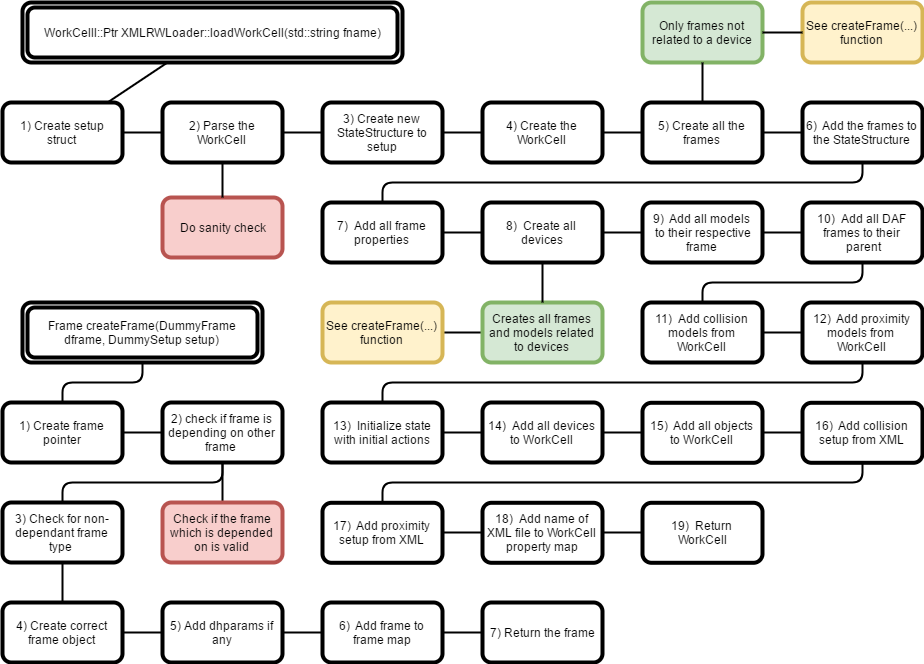
\includegraphics[scale=0.55]{Figures/ComplexLoadWC.png}
	\caption{Illustration of how XMLRWLoader loads the contents of an XML file contianing the description of a WorkCell}
	\label{fig:ComplexLoadWC}
\end{figure}

The XMLRWLoader also implements a helping struct that is called DummySetup, which task is store information related to the setup. This include several maps related to frames, the world frame of the WorkCell, the state structure of the WorkCell, a map related to objects, a vector contain initial actions, the DummyWorkCell, a map containing the devices, a scene descriptor, collision and proximity setup.

\subsection{Implementation of the loader}
The implementation of the loader can be explained in the different capabilities that were added as time went on. The first capability of the loader was to add a device to the WorkCell. The second capability was to be able to give the device a name. The third capability was to be able to apply a transform to the device. The last capability added was the ability to define the parent frame of the device. After all of these capabilities were implemented, the loader now complies with requirements for inserting a device (See need to have requirement 3).

\subsubsection{Adding a device to a WorkCell}
Starting with the loadWorkCell function as a template, the place were the code handles what WorkCell is worked in needs to be rewritten. One of the first things that happen in the loadWorkCell function is that the DummySetup gets a new scene descriptor. This is changed so that the scene descriptor is set to the one from the defined WorkCell. The next thing related to the WorkCell is the state structure and world frame in the DummySetup. The loadWorkCell function normally creates a new state structure and then uses the root of this object as the world frame. this is changed so that the DummySetup is supplied the state structure and the world frame of the defined WorkCell. Lastly the loadWorkCell function creates a new WorkCell, this is simply just removed since it is no longer relevant. Figure~\ref{fig:ChangedInLoaderWorkCell} shows the changes made to the loadWorkCell template in order for it to support defining a WorkCell.

\begin{figure}[h]
	\centering
	\lstset{language=C++} 
	\begin{lstlisting}[frame=single]
	DummySetup setup;
	
	/// XMLRWLoader
	// New scene descriptor is created
	setup.scene = ownedPtr(new SceneDescriptor());
	
	// New State structure is created
	setup.tree = new StateStructure();
	// World frame is saved in setup
	setup.world = setup.tree->getRoot();
	
	// New WorkCell is created using the parsed information
	WorkCell::Ptr wc = ownedPtr(new WorkCell(
		ownedPtr(setup.tree), setup.dwc->_name, fname));
		
	// Scene descriptor of WorkCell is set to that in the setup
	wc->setSceneDescriptor(setup.scene);
	
	
	/// Changes	(wc is the supplied WorkCell)
	// Scene descriptor in setup is set to that of the WorkCell
	setup.scene = wc->getSceneDescriptor();
	
	// Get state structure from the WorkCell
	setup.tree = wc->getStateStructure().get();
	// Get World frame from the WorkCell
	setup.world = wc->getWorldFrame();
	\end{lstlisting}
	\caption{Code example showing changes made to the template from the loadWorkCell(...) function regarding the WorkCell}
	\label{fig:ChangedInLoaderWorkCell}
\end{figure}

\subsubsection{Custom naming the device}
In order to choose the name of the device without, we need to access the information regarding the device and its frames before the device and its frames are created. Luckily, it is already known that this information is situated in the DummyWorkCell. The DummyWorkCell contains a vector with the description of all of the devices, however taken into account how this functionality is going to be used we assume there is only one device description and that there is one. This description of the device contains the name which is simply changed into the wanted name.\\

The name of the frames however is the same which is a problem in the case that one would like to include more then one of the same device. In order to solve this a naming convention for frame names was decided on. The standard naming convention includes the device name and a string describing the frame for the individual frame. As an example, the base frame of a FANUC LRM200 would be named "LRM200.Base". The new naming convention follows this one with the modification that the custom name does not overwrite the device name. It is instead added to the existing name of the frame, preserving the information of the device for the user. Again using the FANUC LRM200 as an example, the new name for the base frame, where the FANUC LRM200 device was named test, would be "test.LRM200.Base".\\

In order to implement the new naming convention for the frames, each frame description contained in the description of the device needs to be accessed. The frame descriptions are contained in a vector in the devices descriptions which is iterated through using a simple for loop. Changing the name of the frame is a little different then with the device since the name of a frame consists of two parts, a scope and the actual name of the frame. In the case of the example earlier with "LRM200.Base", the "LRM200" part would be the scoped part and the "Base" part would be the actual name. Luckily for us the scoped is a vector of strings and the problem s solved by simply adding the name to this scope.\\

Some new problems now arise. First of all the parent frames for frames which name we changed does no longer point to the right frames any more. In the frame description this is called the reference frame and is a string reflecting the name of the parent frame. This needs to be updated to the new name of the frame. This does not apply to the base frame of the device. The base frame has a parent frame which name has not been changed, since the parent is not part of the device. The name of the parent is contained in a single string so the scoping is applied manually.\\

Another problem is that the models are saved in a map uses a string containing the name of the frame the model is associated with. This name also needs to be changed since this contains the old name of the frame. First, all of the models is saved along with the name of the associated frame. The models are then removed from the map and inserted again with the the correct name of the associated frame. This problem is the same for a map containg information about limits and a map containing information about properties. The problem is solved the same way as with the models.\\

The last problem is the collision setup. Much like with the models, the problem here is that the name of the frames in the description are not corrected. The intuitive way of understanding what problem this courses is to imagine the device as a set of geometries. When drawing the device it is inevitable that these geometries collide. In RobWork this courses a collision between the geometries that make up the device. In order for this not to happen, the geometries that makes up the device are excluded in the collision detection. This is done with the frame names which, after the renaming, are wrong. In order to fix this problem the exclude list is extracted from the collision setup and the frames are renamed in a similar fashion to the way done with the models. In order to add the changes to the collision setup in the WorkCell, the two collision setups are merged using the member function merge(...) from the collision setup.

\subsubsection{Adding a transform to the device}
Adding a initial transform to the device is relatively simple as long as a handle to the device is available. This handle is gotten by using the name of the device to extract the newly inserted device from the WorkCell. The transform supplied by the user is then applied to the base of the device. The transform can be given in two ways, as a Transform3D object or as the x, y, z and R, P, Y values. In the case that the x, y, z and R, P, Y values are supplied, the loader calculates the transform from these values using the creator (see chapter~\ref{subsec:iframAGeomUsing}).

\subsubsection{Defining the parent frame for the device}
Changing the parent for the device has a really simple solution. Remember when renaming the device, it was figured out that the reference frames (parent frames) were stored in a string in the frame description. The reference frame for the base of the device is just another way of saying the parent frame for the device. Hence all that needs to be done to solve this problem is to find the description for the base frame and change the reference frame to the defined parent frame.


\subsection{The future of the loader}
As the reader might already have suspected, the loader can be used to add much more than a device. In the case that a XML file with the contains more than a single device, all the other items are also added. This can in some cases be useful, it is however this makes it less intuitive to use the loader. Because of this, one of the more immediate additions to the loader would be to flesh out the functionalities and add catches so the user cannot use the function in an unintended way. The functions, as an example, could be addDevice(...) which adds a single device, addObject(...) which adds a single object described in a XML file and addWC(...) which would add the entire content of another WorkCell described in a XML file to another WorkCell.\\
The reader might also have noticed that when inserting single device, a lot of the actions taken are never used. A good example is the first step in where the frames not associated with a device. This step is unnecessary since there should be none of these frames in the description of a single device. Since the plan would be to create specialized functions, these functions could be optimized by removing the unnecessary parts of the functions.
